\chapter{System Implementation}\label{chap:3}
(Forse posso inserire capitolo in cui illustro anche le componenti software da un punto di vista piu' generico. Ovvero ROS e Dynamixel SDK/workbench. Ho paura non ci si tutto sto granche' da dire, vedremo.)
Now that we have all the theoretical and practical elements of the system, here we report all the work done to implement it on a software side. That includes code written from scratch and also code used to interface with already existing parts. This chapter can be divided in 3 parts: first, we describe the code implemented to control the turret and the solution adopted to overcome the issues mentioned in \ref{subs:firstModel:issues}. Then, we explain how we interface with the arm pointing system and the relative localization procedure. Finally, we describe the implementation of the demos involving the kobuki. Experiment setups and procedures are left for chapter \ref{chap:4}.
\section{Turret Software Implementation}
First, we must recall what are our goals. We want to be able to drive a laser dot on a given surface (i.e. the floor) by setting its \emph{x} and \emph{y} coordinates (the \emph{z} would be implicit on the floor). This must be done with a good precision and also with high frequency, as we want to draw nice and smooth trajectories with the laser. To do so, we can only control two Dynamixel servos, setting their angles values accordingly to the inverse kinematics solved in \ref{sec:1.1}.\\
So, we will describe how we implement the turret model and then the interface written to control the motors and achieve our goals.
\subsection{Turret Model Implementation}
The code to implement the two turret models can be found inside \textbf{tf\_broadcaster.py} and \textbf{mx64\_tf\_broadcaster.py} in the project repository RIFERIMENTO. They implement a ROS node containing the inverse kinematic equation and the code to publish the \emph{tf tree} of the turret. Those models, in fact, are simply implemented as a chain of \emph{tf frames}. \textbf{tf} is a package that lets the user keep track of multiple coordinate frames over time. \textbf{tf} maintains the relationship between coordinate frames in a tree structure buffered in time, and lets the user transform points, vectors, etc between any two coordinate frames at any desired point in time. In that way, we can easily keep track of the position/transformation of our frame, corresponding to our \emph{pan} and \emph{tilt} angle. This is an immediate implementation of the logic already depicted in figures \ref{fig:firstModelRefFrame} and \ref{fig:secondModelRefFrame}. Listing \ref{lst:mx64_tf_broadcaster} shows an example of the code publishing the \emph{tf tree}.\\
So, those are the nodes in charge to compute and keep track of the values of our two DoF.
\begin{lstlisting}[caption={tf tree publisher of the MX-64 based turret},label={lst:mx64_tf_broadcaster},language=Python]
def publish_tf_tree(self, m1, m2):
        self.br.sendTransform((0, 0, dz_to_motor_1_flange),
                         tf.transformations.quaternion_from_euler(0, 0, m1),
                         rospy.Time.now(),
                         "pan_link",
                         "base_link")
        self.br.sendTransform((0, 0, dz_to_motor_2_flange),
                         tf.transformations.quaternion_from_euler(np.pi/2, -np.pi/2, 0),
                         rospy.Time.now(),
                         "tilt_link",
                         "pan_link")
        self.br.sendTransform((0, 0, 0),
                         tf.transformations.quaternion_from_euler(0, 0, m2 - np.pi/2),
                         rospy.Time.now(),
                         "laser_pointer_link",
                         "tilt_link")
        self.br.sendTransform((0.075, 0, 0),
                         tf.transformations.quaternion_from_euler(0, 0, -np.pi/2),
                         rospy.Time.now(),
                         "laser_link",
                         "laser_pointer_link")
        self.br.sendTransform((5.0, 0, 0),
                         tf.transformations.quaternion_from_euler(0, 0, 0),
                         rospy.Time.now(),
                         "debug_link",
                         "laser_link")
        self.rate.sleep()
\end{lstlisting}
\subsection{Motors Controller}
The drivers for both the AX-12+ and the MX-64 Dynamixels are provided by the \textbf{dynamixel\_sdk}. Moreover, the \textbf{dynamixel\_workbench} offers ROS interfaces to work with the official sdk. That is one of the most crucial part of software, because it is directly related to the issues mentioned in section \ref{subs:firstModel:issues}. As a matter of fact, we tried many different solution to overcome our imprecision and trajectory smoothness problem:
\paragraph{ROS Library:} changing the library for ROS, using both official and unofficial;
\paragraph{Wheel Mode vs Joint Mode:} those servos have the possibility to directly control their velocity (wheel mode) and not their position (joint mode, default behaviour). Thus, we implemented an open loop controller in wheel mode;
\paragraph{PID Controller:} again using wheel mode, we tried to build a PID controller;
\paragraph{PID, Joint Mode:} we even tried a PID controller in joint mode, though it did not make much sense;
\paragraph{Compliance Slope and Margin:} those servos have two internal parameters. \emph{Compliance} is to set the control flexibility of the motor.
Diagram in figure \ref{fig:compliance} shows the relationship between output torque and position of the motor. \emph{Compliance Margin} exists in each direction of CW/CCW and means the error between goal position and present position. The greater the value, the more difference occurs. \emph{Compliance Slope} sets the level of Torque near the goal position, the higher the value, the more flexibility is obtained.
\begin{figure}
	\centering
	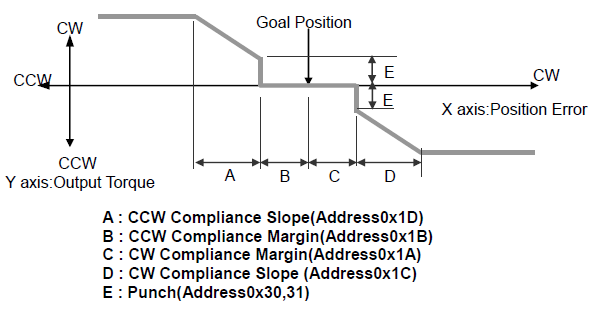
\includegraphics[width=\textwidth]{img/compliance.jpg}%
	\caption{Compliance Slope and Margin}
	\label{fig:compliance}
\end{figure}
\\

All those attempts failed! This is mostly due to the slow communication protocol. As a matter of fact, we found out that the motors were not able to process all the points composing the trajectory that we needed to send at 50Hz and they were simply dropping them. That happens because each time a command is sent through the bus interface, each motors has to send its acknowledgment. So, we disabled all kind of response from the servos, assuming that once a command is sent, it will be properly executed. Moreover, we had to modify the drivers to be sure that the PC would not wait for motors replies. That was a bit tricky as, even though the low level function to write the servos registries without wait for reply existed, we had to find and expose it through the workbench libraries.\\
After that, we were able to draw our smooth trajectories in the simplest way possible: sending points at a fixed rate with the servos in joint mode. That worked fine with the first turret model, but also with the second one. Even better, the \emph{MX-64} based turret worked perfectly thanks to its better resolution.\\

We should mention that the code in charge of interfacing with the motors (i.e. setting the joints position) can be found inside \textbf{dynamixel\_turret.py} for the first model and \textbf{mx64\_turret.py} for the second. Even if they could use the same interface, we have two different file as, for the second turret, the code was rewritten to directly exploit the ROS service interface offered by the \textbf{dynamixel\_workbench}.\\
Finally, inside the \textbf{trajectory\_publisher.py} we have the code to publish the points composing the desired trajectory (e.g. circle, square, \virgolette{$\infty$} shape). 